% !TEX root = ../main.tex
\section{Preprocessing and Validation of Collected Data}

	\todo[inline, color=orange!80]{Bruk dataene her til et avsnitt i diskisjonen om hvor gyldig dataene er.}

	\subsection{Preprocessing of data}
		\todo[inline, color=blue!60]{Skrive litt om hvordan jeg har håndtert rådata. Hvilke verdier er inkludert, hvilke er utelukket, osv. Litt om tomme svar, etc.}

    \begin{figure}[H]
      \centering
      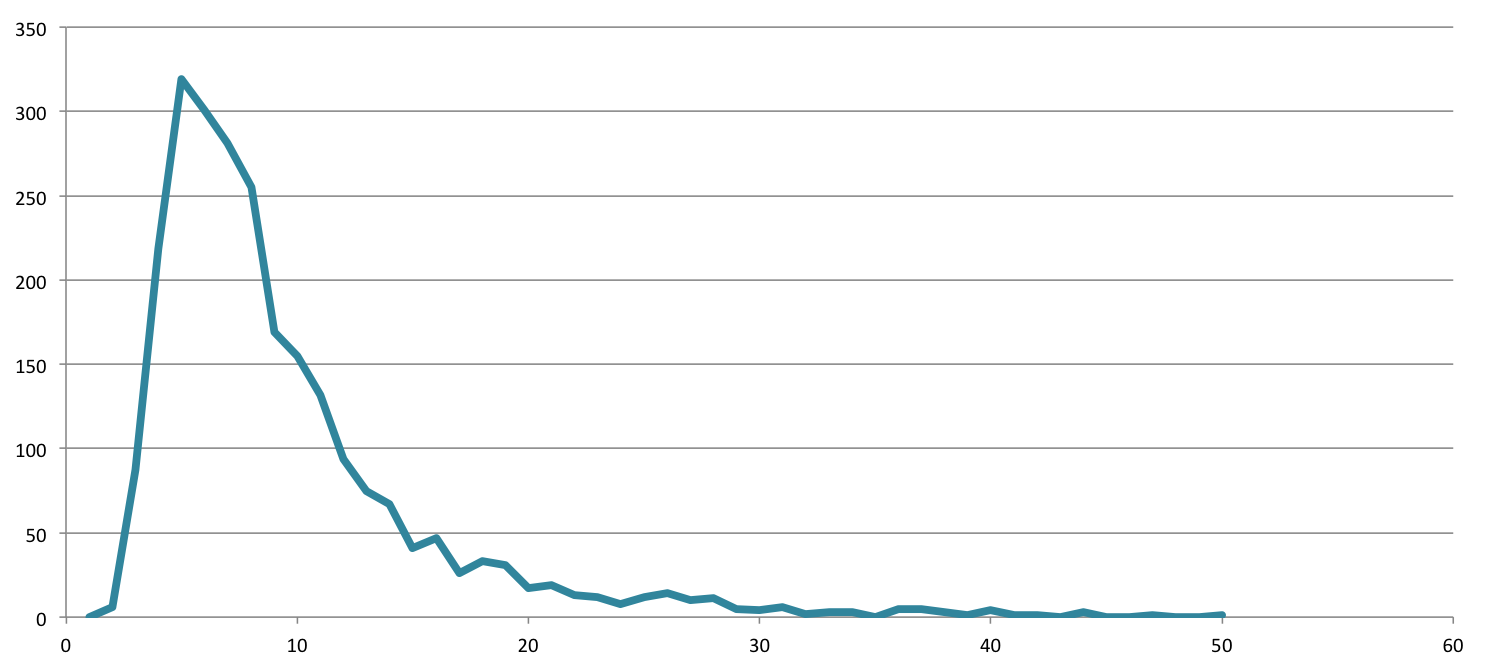
\includegraphics[width=\textwidth]{pics/analysis/limittimeframe.png}
      \caption{Defining max pattern creation time}
    \end{figure}

	\subsection{The Impact of Using Latin Square} \label{sec:latinsquareimpact}

    \todo[inline, color=orange!80]{Se om rekkefølge på mønster har noe å si}

		%Figure: Percentage of times the pattern orders occurred
		\begin{figure}[H]
      \centering
      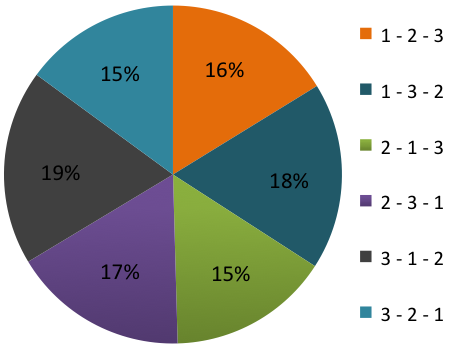
\includegraphics[scale=0.5]{pics/analysis/patternOrder.png}
      \caption{Percentage of times the pattern orders occurred}
      \label{fig:patternOrder}
    \end{figure}

  \subsection{Classification of Handsize and Screensize} \label{sec:classificationhandsizescreensize}

    \subsubsection*{Classification of handsize}
    To be able to analyses if there is a correlation between handsize, screensize, and finger used on the patterns created it is important to validate the subjective parameters handsize and screensize. There is no easy way to ask a person these questions over a survey, so based on the answers I have to validate the answers and decides if they are reliable enough to be further used in a analysis. 

    Handsize should be measured correctly in cm to be able to correctly classify the handsize, but it should not be a requirement that respondents have any tools available to measure their handsize, nor can I ensure that actually measure their handsize correctly. 


		%Figure: Handsize
		\begin{figure}[H]
      \centering
      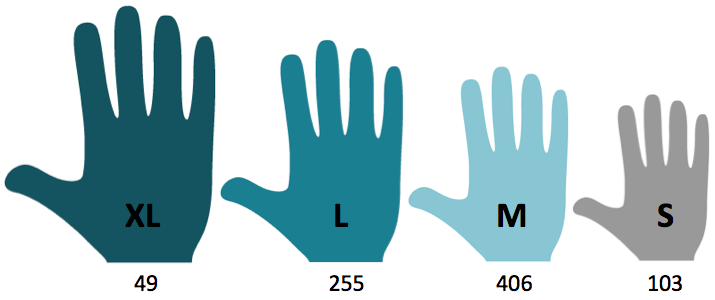
\includegraphics[width=0.8\textwidth]{pics/analysis/handsize.png}
      \caption{Handsize of all participants}
      \label{fig:handsize}
    \end{figure}

    %Table: Handsize and gender
    \begin{table}[H]
      \centering
      \begin{tabular}{ c || c | c | c | c || c }
        \hline
        & {\bf Xtra Large} & {\bf Large} & {\bf Medium} & {\bf Small} & {\bf Total}\\ \hline
        {\bf Male} & 45 (9\%) & 200 (38\%) & 246 (47\%) & 38 (7\%) & 529 \\
        {\bf Female} & 3 (1\%) & 54 (19\%) & 157 (56\%) & 64 (23\%) & 278 \\ \hline
      \end{tabular}
      \caption{Handsize and gender}
      \label{tab:HandsizeGender}
    \end{table}

    Based on own experiences, there is a difference in how the two genders will classify their own handsize. In society, men are supposed to be masculine where big hands are often associated with masculinity. The opposite of masculine, femininity, are associated with smaller hands. It it therefore believed that men will classify their hand as medium or large, while women want to classify their hand as small or medium. The question in survey were asking the participants to select their handsize based on their own gender, but Table \ref{tab:HandsizeGender} confirms that the classification are biased. The majority of the men classified their hand as medium or higher, while women classified their handsize as medium or lower. 

    To be able to cope with the differences, Table \ref{tab:classificationhandsize} are created to match female and male handsize against each other. For example, a male participant classifying their hand as small would probably have bigger hand than a female participant classifying her hand as small. 

    %Table: Classification of handsize
    \begin{table}[H]
      \centering
      \begin{tabular}{ c || c | c | c | c | c }
        \hline
         & {\bf XL} & {\bf L} & {\bf M} & {\bf S} & {\bf XS} \\ \hline\hline
        {\bf Male}   & XL & L  & M & S &   \\
        {\bf Female} &    & XL & L & M & S \\ \hline
      \end{tabular}
      \caption{Classification of handsize for both male and female participants}
      \label{tab:classificationhandsize}
    \end{table}

    \subsubsection{Classification of screensize}

    \todo[inline, color=blue!60]{Må legge til noe oppsummerende tall som beviser at Android phones ikke kan bli klassifisert}

    Classification of screensizes are a hard job due to the problem of various screen sizes and resoulutions across mobile brands. Smartphones operating on Android operation system are known to have a high variation in screen resolutions. The data collected from the mobile survey application are collected from the client, making it impossible to obtain the correct sceeensize of the respondent because it is only possible to obtain the screensize in pixels. The physical size of a mobile screen is not correlated with the pixel size. Apple have standardized the screensizes, making it possible to obtain the physical size of the respondents using a iPhone. The standarized screensizes are shown in Figure \ref{fig:iphonescreenresolutions} and Table \ref{tab:iphonescreen}.

    %Figure: Iphone screen resolutions
    \begin{figure}[H]
      \centering
      \subfigure[iPhone 3.5"]{
        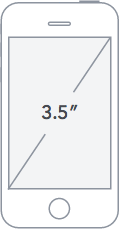
\includegraphics[scale=0.45]{pics/analysis/iphone35.png}
        \label{fig:iphone35}
      }
      \subfigure[iPhone 4"]{
        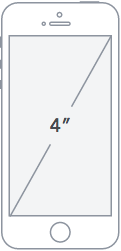
\includegraphics[scale=0.45]{pics/analysis/iphone4.png}
        \label{fig:iphone4}
      }
      \subfigure[iPhone 4.7'']{
        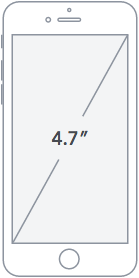
\includegraphics[scale=0.45]{pics/analysis/iphone47.png}
        \label{fig:iphone47}
      }
      \subfigure[iPhone 5.5'']{
        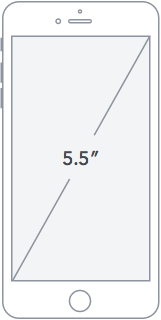
\includegraphics[scale=0.45]{pics/analysis/iphone55.png}
        \label{fig:iphone55}
      }

      \caption{iPhone screen resolutions}
      \label{fig:iphonescreenresolutions}
    \end{figure}

    There are only 4 physical screensizes used on iPhones illustrated in Figure \ref{fig:iphonescreenresolutions}. In my dataset there are only obtained the pixel sizes of the screen where 4 different types were obtained. The subjective answer and the corresponding pixel size are illustrated in Figure \ref{fig:iphoneScreenDist}. Looking at Table \ref{tab:iphonescreen} we can see that there are two resolutions that have a unique correspondence to a physical size, 320$\times$480px  and 414$\times$736px. There are two sizes that correspond to two different physical sizes because iPhone 5 and 6 can both have the screen resolutions 320$\times$568px while iPhone 6 and 6+ can both have the screen resolution 375$\times$667px. Table \ref{tab:iphonescreen} contains a purposed size for each model. There do not exist any scale defining mobile screens from S-L, so this is my own subjective classification of the screensized based on the most popular screensizes on the market. Because of the two overlaps, the 320$\times$480px can be both small or medium, and 414$\times$736px can be both medium and large.

    Comparing my own subjective meaning in Table \ref{tab:iphonescreen} and the subjective classification of the respondents in Figure \ref{fig:iphoneScreenDist}, I will try to make an conclusion if the data are valid for further use. 

    The smallest screen resolution, 320$\times$480px, do have very different subjective meaning of the screensize. Comparing the different models with that size with the other models, the screen can be classified to have a small screensize. It looks promising that none of the respondents classified 320$\times$480px as a large screen. The next screen resolution is the 320$\times$568px. The most of the participants have classified the smartphone as small, while the majority have classified the screen as medium. The only possible iPhones that can have that size is the iPhone 5 and 6 that have a medium screensize compared to other models. There are also none of the respondents classifying the screen resolution 320$\times$568px as a large screen. The next is rather hard to precisely classify because the 375$\times$667px can be both an iPhone 6 or 6+. iPhone 6 are compared to other models a medium screen while iPhone 6+ are one of the biggest screens in the market, making iPhone 6 a medium screen and iPhone 6+ as a large screen. The 3 respondents classifying the 375$\times$667px screen as small screen can be moved up to a medium screen. The last screen resolution, 414$\times$736px, can we just define as a large screensize because the only iPhone having this size is the iPhone 6+. 

    %Figure: Iphone screensize distribution
    \begin{figure}[H]
      \centering
      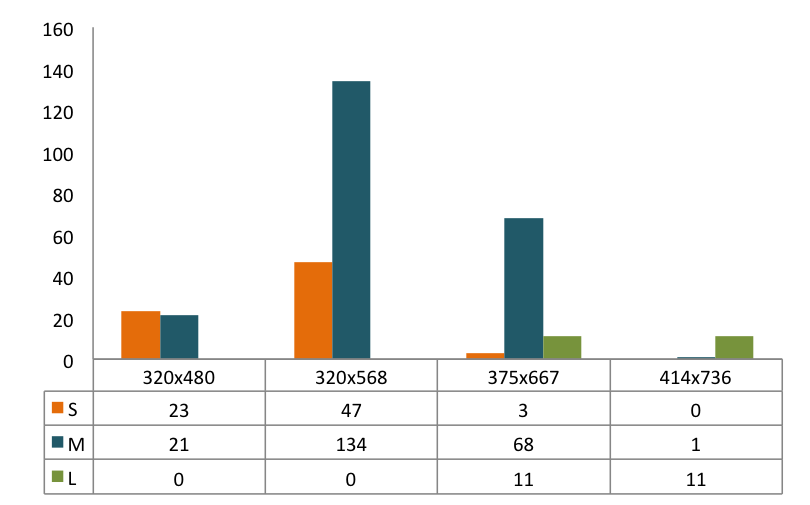
\includegraphics[scale=0.85]{pics/analysis/IphoneScreenDist.png}
      \caption{Iphone screensize distribution}
      \label{fig:iphoneScreenDist}
    \end{figure}

    %Table: Iphone Screen classification
    \begin{table}[H]
      \centering
      \begin{tabular}{ l | l | l | l }
        \hline
        {\bf Iphone Model}  & {\bf Resolution (px)} & {\bf Inches} & {\bf Size} \\ \hline
        iPhone 2G, 3G, 3GS, 4, 4s  &  320 $\times$ 480  &  3.5'' & S\\
        iPhone 5, 5s        &  320 $\times$ 568  &  4'' & M \\
        iPhone 6            &  320 $\times$ 568, 375 $\times$ 667  &  4.7'' & M/L \\
        iPhone 6 Plus       &  375 $\times$ 667, 414 $\times$ 736  &  5.5'' & L \\ \hline        
      \end{tabular}
      \caption{Iphone screensizes}
      \label{tab:iphonescreen}
    \end{table}

    \todo[inline, color=blue!60]{Legge til en konklusjon om man kan stole på resultatene (bare iphones) og om de kan brukes videre i en analyse.}

  \subsection{Validity}

    \todo[inline, color=red!80]{Internal and external validaty}